\documentclass{beamer}
\usepackage[utf8]{inputenc}

\usetheme{Madrid}
\usecolortheme{default}
\usepackage{amsmath,amssymb,amsfonts,amsthm}
\usepackage{txfonts}
\usepackage{tkz-euclide}
\usepackage{listings}
\usepackage{adjustbox}
\usepackage{array}
\usepackage{tabularx}
\usepackage{gvv}
\usepackage{lmodern}
\usepackage{circuitikz}
\usepackage{tikz}
\usepackage{graphicx}

\setbeamertemplate{page number in head/foot}[totalframenumber]

\title{2.10.30}
\date{September 19, 2025}
\author{EE25BTECH11001 - Aarush Dilawri}

\begin{document}

\frame{\titlepage}

\begin{frame}{Solution}
We have position vectors
\begin{align}
\vec{A} &= \myvec{60 \\ 3}, \quad 
\vec{B} = \myvec{40 \\ -6}, \quad 
\vec{C} = \myvec{a \\ -52}.
\end{align}
\end{frame}
\begin{frame}{Solution}
    Now,
    \begin{align}
    \vec{B} - \vec{A} &= \myvec{-20 \\ -9}, \\
    \vec{C} - \vec{A} &= \myvec{a-60 \\ -55}.
\end{align}
\end{frame}
    
\begin{frame}{Solution}
    For collinearity, we require
\begin{align}
    \quad \text{rank}\,\myvec{\vec{B}-\vec{A} & \vec{C}-\vec{A}} = 1
\end{align}
\begin{align}
    \quad \text{rank}\,\myvec{-20 & a-60 \\ -9 & -55} = 1
\end{align}
\end{frame}


\begin{frame}{Solution}
\begin{align}
R_2 &\to R_1 - \tfrac{20}{9}R_2
\end{align}
\begin{align}
\myvec{-20 & a-60 \\ -9 & -55}
\;\xleftrightarrow{\,R_2 \to R_1 - \frac{20}{9}R_2\,}\;
\myvec{-20 & a-60 \\[6pt] 0 & a + \frac{560}{9}}
\end{align}
\begin{align}
    \quad \text{rank}\,\myvec{-20 & a-60 \\ 0 & a + \frac{560}{9}} = 1
\end{align}
\end{frame}
\begin{frame}{Solution}
Therefore, equating the last row to 0, we have
\begin{align}
    a + \frac{560}{9} = 0
    \implies a = -\frac{560}{9}
\end{align}

Therefore, the answer is (d) None of these.
\end{frame}

\begin{frame}{Figure}
\begin{center}
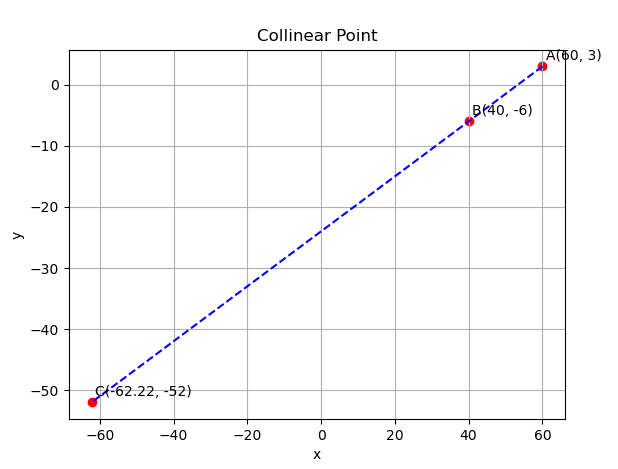
\includegraphics[width=0.6\columnwidth]{figs/fig.png}
\end{center}
\end{frame}
\begin{frame}[fragile]{C Code (code.c)}
\begin{lstlisting}[language=C]
#include <stdio.h>

double find_a(double x1, double y1, double x2, double y2, double y3) {
    double u1 = x2 - x1;
    double u2 = y2 - y1;
    double v2 = y3 - y1;

    double lambda = v2 / u2;

    double a = x1 + lambda * u1;
    return a;
}
\end{lstlisting}
\end{frame}
\begin{frame}[fragile]{Python Code (code.py)}
\begin{lstlisting}[language=Python]
import numpy as np
import matplotlib.pyplot as plt

x1, y1 = 60, 3
x2, y2 = 40, -6
y3 = -52

u1, u2 = (x2 - x1), (y2 - y1)
lambda_val = (y3 - y1) / u2
a = x1 + lambda_val * u1
print("Value of a =", a)

A = np.array([x1, y1])
B = np.array([x2, y2])
C = np.array([a, y3])

\end{lstlisting}
\end{frame}
\begin{frame}[fragile]{Python Code (code.py)}
\begin{lstlisting}[language=Python]
plt.scatter([A[0], B[0], C[0]], [A[1], B[1], C[1]], color="blue")

plt.text(A[0] + 1, A[1] + 1, "A(60, 3)", fontsize=10, color="black")
plt.text(B[0] + 1, B[1] + 1, "B(40, -6)", fontsize=10, color="black")
plt.text(C[0] + 1, C[1] + 1, f"C({a:.2f}, -52)", fontsize=10, color="black")

plt.plot([A[0], B[0], C[0]], [A[1], B[1], C[1]], linestyle="--", color="red")

plt.xlabel("x")
plt.ylabel("y")
plt.title("Collinear Points")
plt.grid(True)
plt.show()
\end{lstlisting}
\end{frame}
\begin{frame}[fragile]{Python Code (nativecode.py)}
\begin{lstlisting}[language=Python]
import ctypes
import numpy as np
import matplotlib.pyplot as plt

lib = ctypes.CDLL("./code.so")
lib.find_a.argtypes = [ctypes.c_double, ctypes.c_double,
                       ctypes.c_double, ctypes.c_double,
                       ctypes.c_double]
lib.find_a.restype = ctypes.c_double

x1, y1 = 60, 3
x2, y2 = 40, -6
y3 = -52

a = lib.find_a(x1, y1, x2, y2, y3)
print("Value of a =", a)

A = np.array([x1, y1])
B = np.array([x2, y2])
C = np.array([a, y3])
\end{lstlisting}
\end{frame}
\begin{frame}[fragile]{Python Code (nativecode.py)}
\begin{lstlisting}[language=Python]
plt.scatter([A[0], B[0], C[0]], [A[1], B[1], C[1]], color="red")

plt.text(A[0] + 1, A[1] + 1, "A(60, 3)", fontsize=10, color="black")
plt.text(B[0] + 1, B[1] + 1, "B(40, -6)", fontsize=10, color="black")
plt.text(C[0] + 1, C[1] + 1, f"C({a:.2f}, -52)", fontsize=10, color="black")

plt.plot([A[0], B[0], C[0]], [A[1], B[1], C[1]], linestyle="--", color="blue")

plt.xlabel("x")
plt.ylabel("y")
plt.title("Collinear Points")
plt.grid(True)
plt.show()
\end{lstlisting}
\end{frame}
\end{document}


